\section{Theory} %\todo{Different name!}
% Beskriv nn. brug nn's problemer til at indroducere rnn
% Beskriv rnn. brug rnn's problemer til at indroducere lstm
% Beskriv lstm

% Hvad er neural network, recurrent nn, lstm
% Tegning/diagram over de forskellige ting - husk at det skal være relevant og skarpt.

\subsection{Neural Network}
% feed forward networks bruges bl.a. til image-recognition	
		
An \gls{ann} is a function that maps an input vector to an output vector. 
It is consisting of layers interacting in some way. A typical \gls{ann} is the \gls{mlp}.
It consists of multiple layers were each layer uses the last layer's output as input.
The combutation that each layer does is multiplying it's input with a weight, adds a bias and applies 
some non-linear activation function. As a function, a \gls{mlp} can be written as:

\begin{align*}
	MLP(x) &= MLP_L(x) \\
	MLP_l(x) &= f(W_l * MLP_{l-1} + b_l) \\
	MLP_0(x) &= x
\end{align*}

where $w_l$ is a weight matrix, $b_l$ is a bias vector and $L$ is the number of layers after the 
input layer, if $L=2$ it is a shallow network with only one hidden layer and if greater it is a deep network
with multiple hidden layers.

The \gls{mlp} is multiplying the input by some weight matrix that cannot change dimensions from input to 
input, it therefore requires that the input have some fixed length. This can give difficulties with 
problems where instances is sequences of different lengths. Different techniques, each with it's own 
shortcomings, can be used to apply \glspl{mlp} in such areas. 
Two typical ways to do this is with a sliding window or with some sort of feature extraction or 
a combination of the two. If the wanted output for the sequence is fixed length, like a classification, 
% TODO like in tmseg step3, "is the seqment a tmh or not
one can transform the input sequence to some fixed length by extracting the most important information
from it. A problem with this is that some information has to be discarded and it is not always 
obvious to see which features is the important ones, this usually require export knowledge in the
field from with the problem originates. 
If the wanted ouput is on the other hand a sequence, a sliding window can be used. 
This is done by taking a fixed length segment of the sequence and using that as input to compute 
a fixed length segment of the output and then moving the window by some amount in the sequence and compute 
a new segment of the output, this is then repeated until the window has sled through the whole sequence.
An advantage with this technique is no information is thrown away, but if some part of the output is 
dependent on different parts of the input, it can be hard to chose a window length that 
encapsulate all part of the input that it depends on, this can be remedied by augmenting 
the window with features extracted from the whole sequence, but this involve the same problems 
from before.
	
\subsection{Recurrent Neural Network}

A \gls{rnn} is a network that besides the input also uses the output from last time it was computed 
as seen in Figure \ref{fig:rnn}.
This recurrent connection enables the network to remember what it has seen previous.

\begin{align*}
	h_t &= A(x_t, h_{t-1}) \\
	h_0 &= initial\_state
\end{align*}

where $t$ is the time step and $A$ is some neural network function. In a standard \gls{rnn} this 
function is just a single layer from a \gls{mlp}.

\begin{figure}
	\centering
	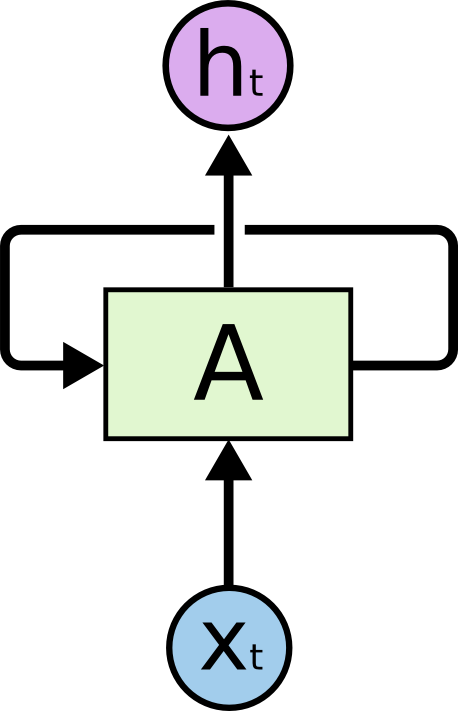
\includegraphics[width=5em]{sections/theory/RNN-rolled.png}
	\caption{A recurrent neural network uses the output as input 
		and has some neural network. Illustration is from \cite{rnn}}
	\label{fig:rnn}
\end{figure}

This sort of network can be used directly on sequence data by using each element in the sequence as
an input to the network as different time steps, $x=x_1x_2...x_t$. The output can then be a sequence 
by using all output, $h=h_1h_2...h_t$, or for classification the last output can be used. 
As seen in Figure \ref{fig:rnn-seq}

\begin{figure}
	\centering
	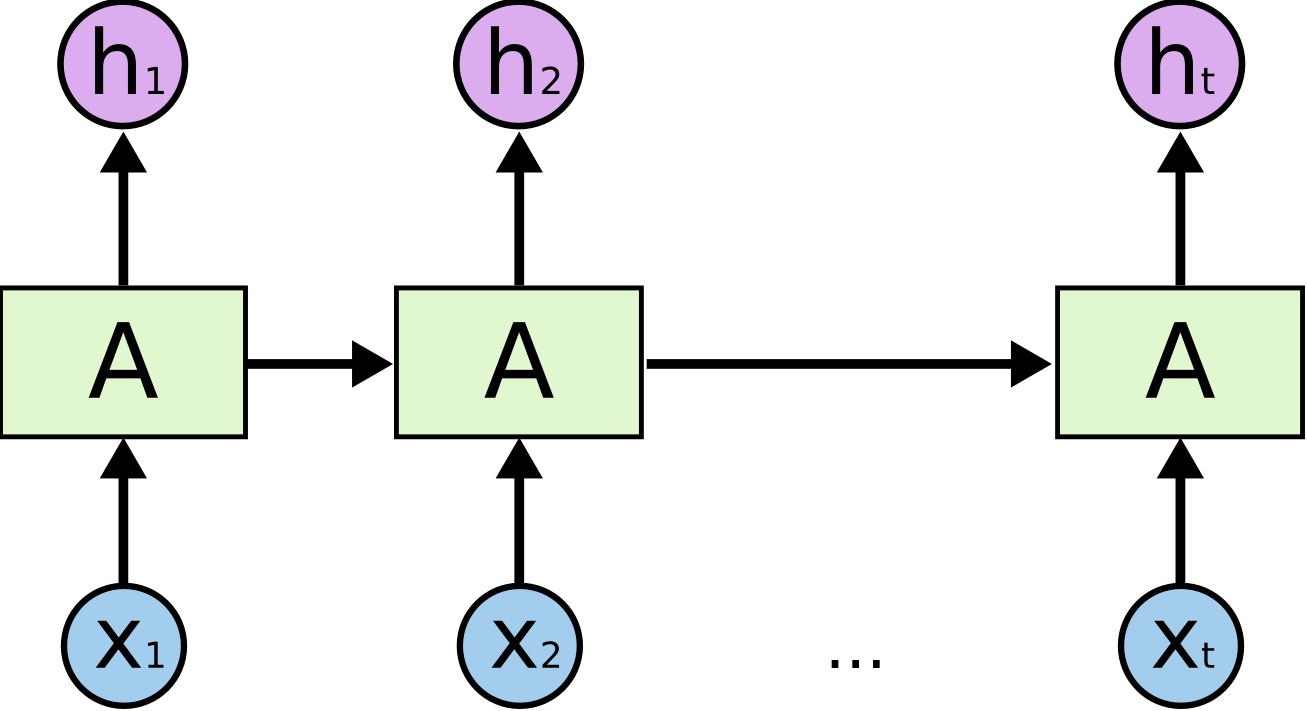
\includegraphics[width=20em]{sections/theory/RNN-unrolled.png}
	\caption{When the input is a sequence, the network becomes a chain of networks 
		as long as the input. Illustration is from \cite{rnn}}
	\label{fig:rnn-seq}
\end{figure}

With this network topology each output point is based on all input seen before and no information is 
chosen beforehand to be thrown away. With a single layer \gls{rnn} only data from one direction can be used
and if output is dependent on data from both directions, a bidirectional layer can be used. This is 
done by running a \gls{rnn} on both directions and concatenate the output at each time step, 
and then have a layer on top of that to uses the information collected from both directions.

In practise it has been shown that it is increasing hard\cite{rnnLTD} to train a \gls{rnn} to 
use information that has an increasing distance in the sequence. This is because the recurrent connection 
is going throug the activation function in each time step and is therefore exhibiting the same vanishing 
gradient problem that very deep feed-forward networks have, which causes the network to not learn 
any long term dependencies. 

\subsection{Long Short-Term Memory Network}
\label{sec:lstm}

A number of different solution to the long-term dependency problem have been proposed and one of the most used
is the \glsfirst{lstm} \cite{lstm}. This is a type of \gls{rnn} where the network function $A$ is more
complicated interaction of four layers, there is also introduced a new recurrent connection called 
the cell-state, $C$. The function then becomes:

\begin{align*}
 h_t, C_t &= A(x_t, h_{t-1}, C_{t-1}) \\
 h_0, C_0 &= initial\_state
\end{align*}

In \glspl{lstm} $A$ is usually called a cell.
The four layers in $A$ consists of three \emph{gates}, $f_t$, $i_t$ and $o_t$, that governs the flow of
information and a cell-state update, $\widetilde C_t$, that updates the cell-state in each time step.
The four layers is:

\begin{align*}
f_t &= \sigma(W_f \cdot [h_{t-1},x_t] + b_f) \\
i_t &= \sigma(W_i \cdot  [h_{t-1},x_t] + b_i) \\
\widetilde C_t &= \tanh (W_C \cdot [h_{t-1},x_t] + b_C) \\
o_t &= \sigma(W_o \cdot [h_{t-1},x_t] + b_o)
\end{align*}

where $W_f, W_i, W_C, W_o$ is weights, $b_f, b_i, b_C, b_o$ is basis', $[h_{t-1},x_t]$ is the 
concatenation of the previous output and the input, and $\sigma$ and $\tanh$ is activation functions.
$f_t$ is called the forget gate and governs how much of the cell-state should be forgotten. 
$i_t$ is called the input gate because it chooses how much new information from the input should
be added to the cell-state. $o_t$ is called the output gate because it governs how much of the 
cell-state should be outputted. The recurrent connections is then calculated by:

\begin{align*}
C_t &= f_t * C_{t-1} + i_t * \widetilde C_t \\
h_t &= o_t * \tanh (C_t)
\end{align*}

An illustration of a cell can be found in Figure \ref{fig:lstm}.
The gates uses $\sigma$ as the activation function because it gives an output between $0$ and $1$
and it can then be interpreted as percentages of information allowed through, it then multiplied
on the vector it governs.

\begin{figure}
	\centering
	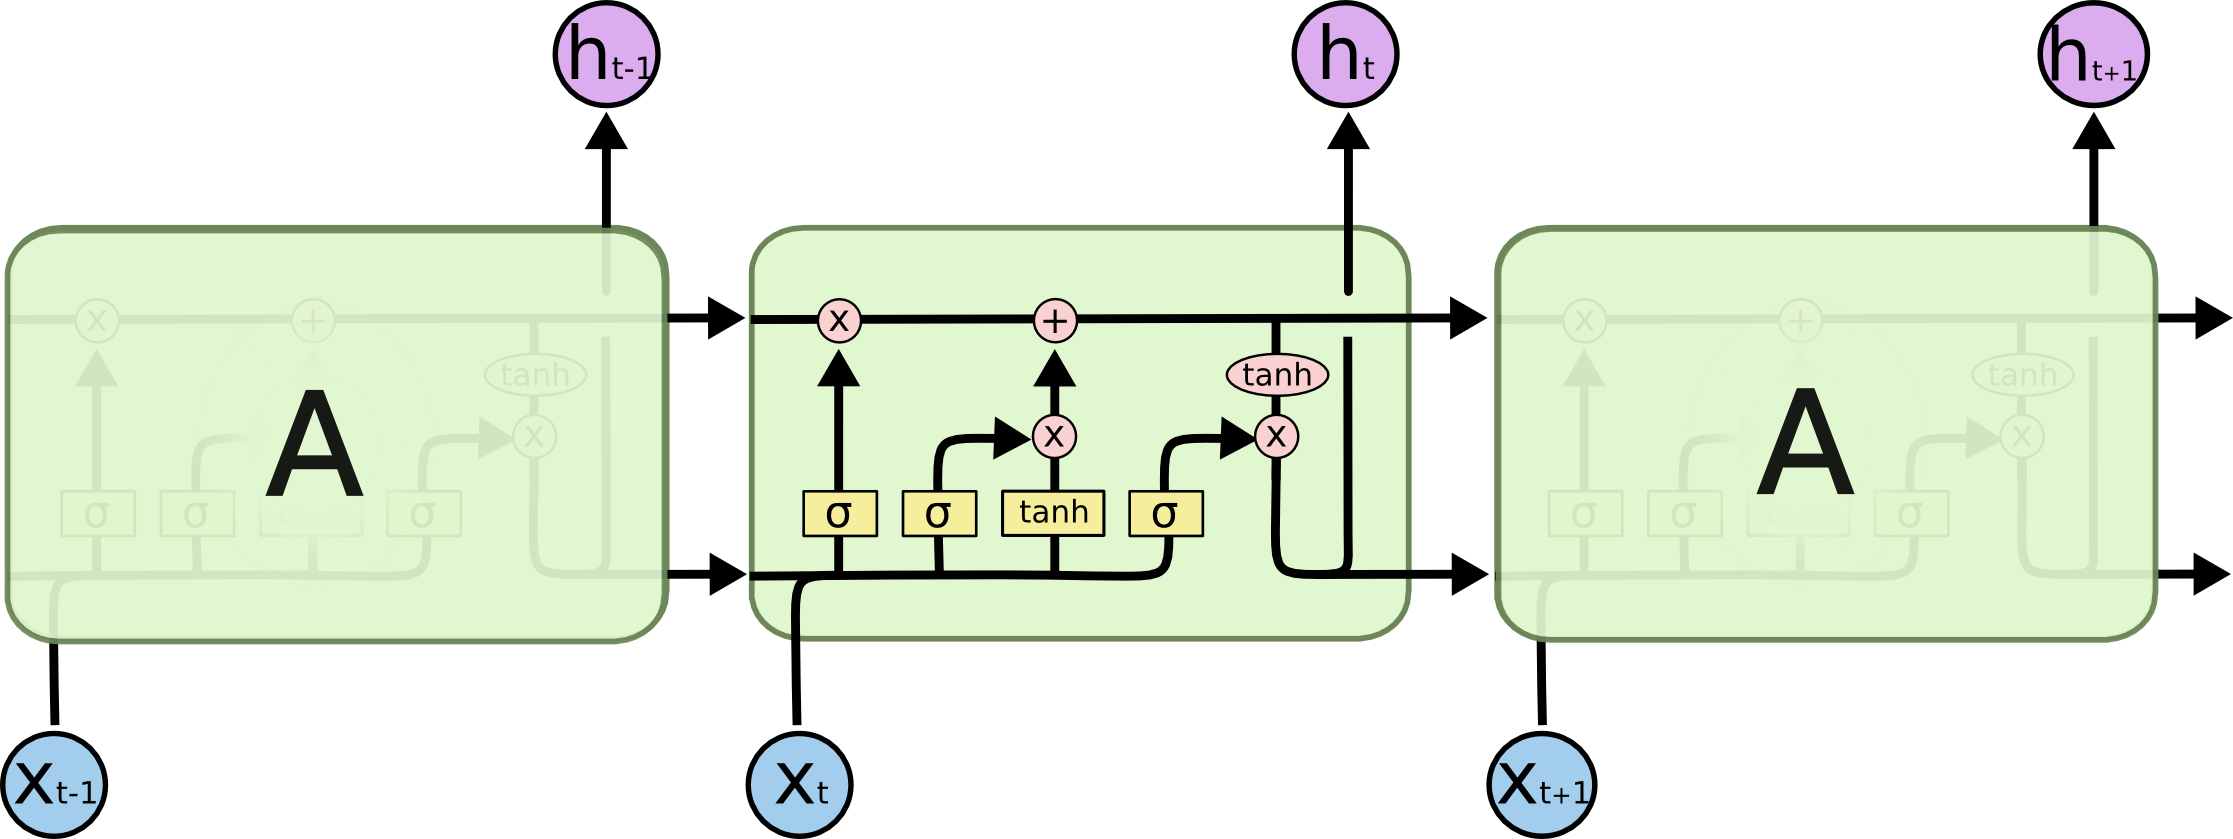
\includegraphics[width=\textwidth]{sections/theory/LSTM3-chain.png}
	\caption{Long Short-Term Memory Networks is a chain of cells, each containing four layers 
		interacting to compute two recurrent connections. Illustration is from \cite{rnn}}
	\label{fig:lstm}
\end{figure}

This type of network does not have the problem of learning long-term dependencies because the depth  
of activation functions from any input to any output is only two, once when the information is 
added to the cell-state and once when the output is calculated, and the gradient is therefore 
much more stable at longer distances in the network. 


